\documentclass[10pt,aspectratio=169]{beamer}
\usetheme{metropolis}
\usepackage{xeCJK}
\setCJKmainfont{FandolSong}
\setCJKsansfont{FandolHei}
\setCJKmonofont{FandolFang}
\usepackage{booktabs}
\usepackage{graphicx}
\usepackage{amsmath}
\usepackage{xcolor}
\definecolor{ok}{HTML}{2E7D32}\definecolor{bad}{HTML}{C62828}\definecolor{hl}{HTML}{B26A00}
\setbeamertemplate{navigation symbols}{}
\setbeamerfont{frametitle}{size=\large}
\title{扩散模型 × 最优传输}
\subtitle{问题 · 理论 · 经典 · 前沿 · 我们能做什么 —— awesome\_diffusion\_OT 综合汇报}
\author{Yufeng Li（asimfish）}
\institute{github.com/asimfish/awesome\_diffusion\_OT}
\date{2026-09-01}
\begin{document}
\maketitle

\begin{frame}{五个问题，五句话}
\small
\begin{tabular}{p{0.2\textwidth}p{0.74\textwidth}}\toprule
问题 & 一句话答案 \\ \midrule
问题是什么 & 生成 = 把噪声/源分布搬到数据分布；路径几何、耦合选择、跨域语义、最优性、计算与统计代价 = P1--P5 \\
别人的理论 & 扩散 = KL 的 Wasserstein 梯度流；SB = 熵正则 OT 的动态形式；FM 与扩散统计等价。「扩散 encoder $\approx$ OT」「拉直 = OT」均被反例证伪 \\
经典工作 & 数学五件套（Brenier / McCann / JKO / Benamou--Brenier / Otto）+ 计算三件套（Sinkhorn / Score-SDE / DSB）+ 范式三线（FM / RF / SI） \\
最新工作 & 理论收口（IMF 指数率、FM minimax、$O(d/T)$、c-RF）· 一步生成新范式 · FlashSinkhorn 拐点 · 桥模型进医学 \\
我们能做什么 & 保边缘噪声指派（\#1，已立项）· OT-aware 调度（\#2）· 保耦合蒸馏（\#3）· 剂量学导向医学 SB（\#7） \\ \bottomrule
\end{tabular}
\end{frame}

\begin{frame}{语料：446 篇是怎么来的}
\begin{columns}
\column{0.5\textwidth}
\begin{itemize}
\item 30 个并行调研 agent（8/14）$\to$ ARIS 三层审计 $\to$ 8/25 复审 $\to$ 9/1 Q3 增量
\item 477 条引用去重 $\to$ \textcolor{hl}{446 篇}，$\star$ 核心 139；345 篇有 arXiv id
\item 证据级 [P] 345 · [A] 24 · [R] 62 · [B] 15
\item NeurIPS 96 · ICLR 80 · ICML 71 · CVPR 29；2024--25 贡献 63\%
\item 每篇：8 节深读（数字带出处）+ 原文 + 保版式译文（对象级 QA）
\end{itemize}
\column{0.5\textwidth}
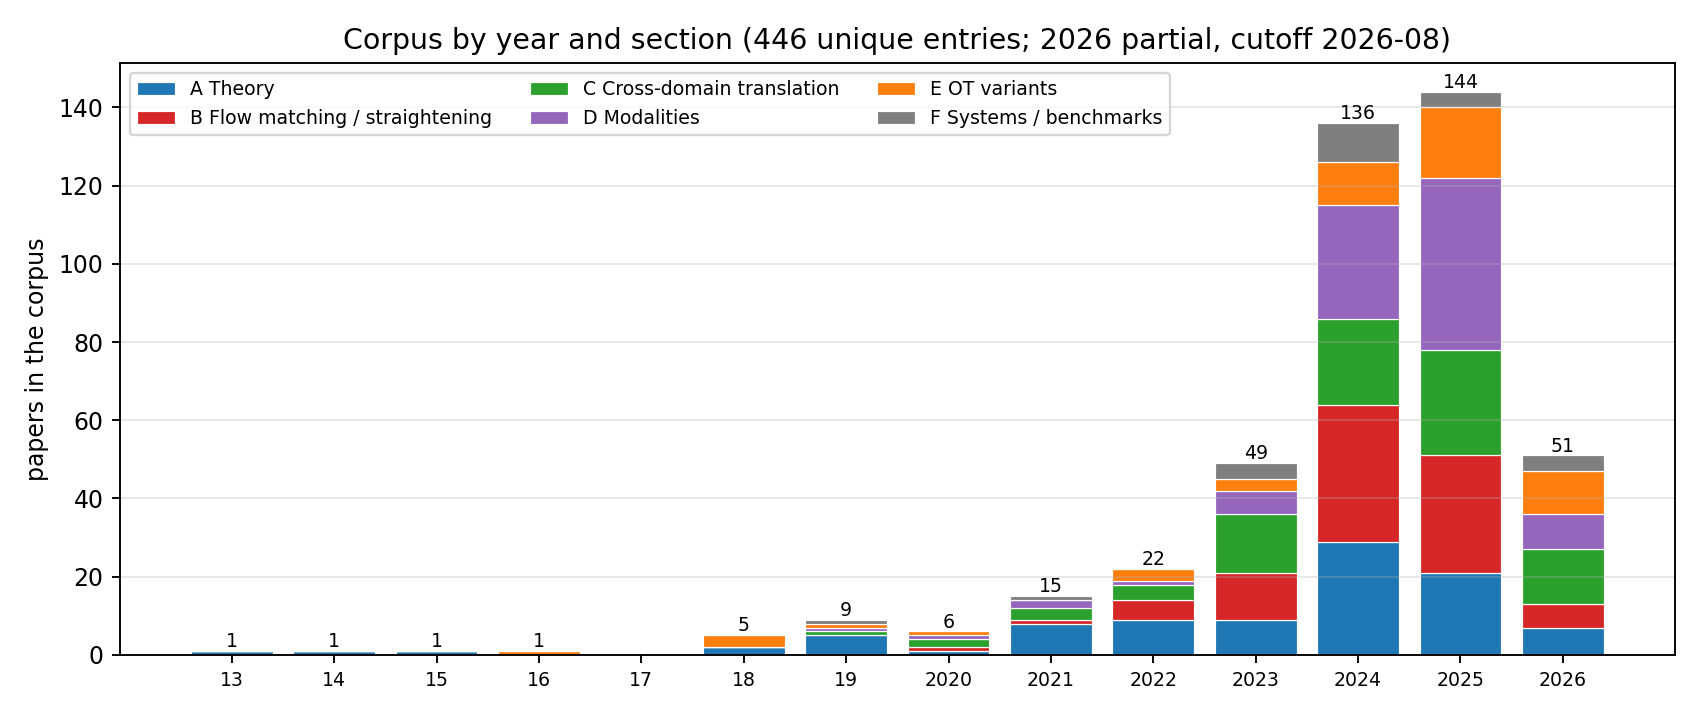
\includegraphics[width=\textwidth]{corpus_by_year.png}
\end{columns}
\end{frame}

\begin{frame}{元问题：生成建模 = 测度传输}
任何生成流的动能 $\ge W_2^2$，缺口就是弯曲程度：
\[ W_2^2(\mu_0,\mu_1)=\min_{(\rho_t,v_t)}\int_0^1\mathbb E_{\rho_t}\|v_t\|^2dt\quad\text{s.t.}\quad\partial_t\rho_t+\nabla\!\cdot(\rho_tv_t)=0 \]
\begin{itemize}
\item \textbf{P1 路径几何}：曲率 $\to$ 离散化误差 $\to$ 最小 NFE；八月：曲率来自去噪器雅可比
\item \textbf{P2 耦合选择}：minibatch OT 受维度诅咒；$n\approx10^6$ 才见收益；\textcolor{hl}{改耦合 vs 保边缘}
\item \textbf{P3 跨域传输}：SB 最正统；深读发现配对桥全部回避耦合学习
\item \textbf{P4 最优性}：高斯成立、一般证伪、量化开放
\item \textbf{P5 计算与统计}：FlashSinkhorn 161$\times$；OT 耦合训练的统计率完全空白
\end{itemize}
\end{frame}

\begin{frame}{两条辩论线都以反例收尾}
\begin{columns}
\column{0.5\textwidth}
\textbf{扩散 $\overset{?}{=}$ OT（T02）}
\begin{itemize}
\item 正方：高斯情形 DDPM encoder = Monge map
\item 反方定论：逐时刻是梯度场，复合后不是凸势梯度（Hessian 非交换项）
\item \textcolor{bad}{缺口未被量化（open problem）}
\end{itemize}
\column{0.5\textwidth}
\textbf{拉直 $\ne$ OT（T09）}
\begin{itemize}
\item RF：保边缘、单调不增凸代价、直线度 $O(1/K)$；直是 $c$-最优的必要非充分条件
\item 反例：迭代 rectification 有非最优不动点（NeurIPS 2025）
\item \textcolor{ok}{八月修复 $\times2$}：c-RF 梯度类投影恒收敛到 OT；reflow$\times$minibatch-OT 极限 = $N$-循环单调耦合
\end{itemize}
\end{columns}
\vspace{4pt}
结论：「直线度」与「最优性」是两个自由度，加一个投影约束就能接上。
\end{frame}

\begin{frame}{四大理论张力（+ 一条工程张力）}
\begin{enumerate}
\item \textbf{耗散 vs 测地}：扩散走 KL 梯度流（JKO），OT 走测地线（BB）
\item \textbf{逐时刻最优 vs 全局最优}：每一瞬是梯度场，复合起来不是
\item \textbf{直 vs 最优}：直线化降代价但不动点未必最优；c-RF / $N$-循环单调条件修复
\item \textbf{加速 vs 统计精度}：各自 sharp，联合前沿无人刻画
\item \textcolor{hl}{\textbf{改耦合 vs 保边缘}}（深读新增）：实例级选择提高兼容性但改变有效初始分布；文献几乎不报告漂移
\end{enumerate}
\end{frame}

\begin{frame}{Schrödinger 桥：五代求解器与 Q3 精细化}
\small
\begin{tabular}{p{0.18\textwidth}p{0.3\textwidth}p{0.46\textwidth}}\toprule
代 & 代表 & 关键洞见 \\ \midrule
1 深度 IPF & DSB · SB-FBSDE & SGM 恰为第一次 IPF 迭代 \\
2 IMF / matching & DSBM · IDBM & SB 是唯一既 Markov 又属 reciprocal 类的过程 \\
3 轻量化 & LightSB(-M) · GSBM & 任意耦合单次 matching 即恢复 SB \\
4 在线/离散/半监督 & $\alpha$-DSBM · CSBM · FSBM & $<8\%$ 配对样本 \\
5 理论收口 & IMF 指数率 · Sinkhorn bridge 统计 & 首个非渐近 KL 指数率 \\
\textcolor{hl}{Q3 新} & PRISM · SDDBMs · 混合分布桥 · 高温 SB & 从「怎么解」到「解什么」 \\ \bottomrule
\end{tabular}
\end{frame}

\begin{frame}{前沿六线（2025--2026）}
\begin{itemize}
\item \textbf{理论收口}：IMF 指数率 · c-RF · 极限点定理 · FM minimax · $O(d/T)$ · SGM = Wasserstein proximal
\item \textbf{一步生成}：MeanFlow（1-NFE FID 3.43）· W-Flow（1.29）· Beckmann 自治流 · LBM
\item \textbf{耦合工程}：大规模 Sinkhorn $\to$ 半离散 $\to$ LOOM $\to$ C$^2$OT $\to$ \textcolor{hl}{QC-FM $O(n)$}
\item \textbf{推理期对齐}（七环节）：NoiseQuery / Golden Noise / verifier 搜索…；\textcolor{bad}{不报告边缘漂移}
\item \textbf{桥与翻译}：UniDB++ · DBIM / CDBM · Q3 新增 11 篇（DoseBridge 以剂量为目标）
\item \textbf{系统与评测}：FlashSinkhorn = attention 同构（仍 [A]）；FID 对少步失真；SynthRAD 教训
\end{itemize}
\end{frame}

\begin{frame}{Q3 增量扫描：62 篇，三条主线}
\begin{itemize}
\item 6 组 arXiv 查询 $\to$ 122 候选 $\to$ 分级 + 人工复核 $\to$ 62 篇（核心 24）
\item \textbf{拉直理论加投影}：c-RF · 极限点定理 $\to$ \#4 降为「实用化空位」
\item \textbf{耦合工程降本}：QC-FM · Gromov-Monge FM
\item \textbf{SB 精细化}：PRISM · SDDBMs · 混合分布桥 · 高温 SB
\item 触发点：ECCV 2026 9/8--12（论文集已上线）· NeurIPS 2026 放榜 9/24 · ICML PMLR 卷未出（FlashSinkhorn 仍 [A]）
\end{itemize}
\end{frame}

\begin{frame}{逐篇深读改变了什么（T14 桥翻译 14 篇为例）}
\begin{itemize}
\item \textbf{随机桥 vs 确定性直线}：I2SB / DDBM / DBIM / LBM 一致——最优噪声强度由任务条件熵与步数预算决定
\item \textbf{配对桥全部回避耦合学习}：DDBM Thm 2 只保边际；CDBM Prop.\,3.2 只保 PF-ODE 解映射；\textcolor{hl}{无一篇陈述蒸馏后终端耦合是否保持}
\item \textbf{横向比较前先统一协议}：E$\to$H 指标在训练集上算；DDBM 的 $N{=}40$ 实为 NFE 118
\item T12：噪声选择文献质量指标齐全，\textcolor{bad}{边缘漂移与多样性无人报告}
\item T09：RF 的 $O(1/K)$ 是对 $\min_k$ 的界且假设精确求解
\end{itemize}
\end{frame}

\begin{frame}{十二条洞察（摘要）}
\small
\begin{enumerate}
\item OT 是设计语言不是自动性质——度量「距 OT 的偏差」
\item 「OT 用量」是精确可研究的变量
\item 免重训的价值集中在耦合与调度两个自由度
\item 直线化与最优性解耦，八月两个定理重新接上
\item 理论骨架收口，论文级空位在接缝处
\item 蒸馏的「保耦合」是零保证地带（深读坐实）
\item 桥模型的最优随机性由任务决定
\item 基础设施拐点已到，多 GPU 空位开放
\item 评测系统性错位，OT 可当解药
\item 高校比较优势区域明确：理论补全 + 接口缝合
\item 医学垂直入场条件已验证，窗口收窄
\item 深读改变了两个 8/25 判断（\#1 卖点降级；\#4 降为实用化）
\end{enumerate}
\end{frame}

\begin{frame}{Top-10 切入点状态（2026-09-01）}
\scriptsize
\begin{tabular}{clll}\toprule
\# & 切入点 & 类型·算力 & 状态 \\ \midrule
1 & 免训练 batch 级保边缘噪声指派（MPNA） & 方法+理论·低 & \textcolor{ok}{已立项 + 沙盒完成} \\
2 & OT-aware 采样调度 & 理论·低 & 空位仍在；曲率来源新刻画 \\
3 & 保耦合的桥蒸馏 + 漂移度量 & 方法·中 & 空位仍在；文献零保证 \\
4 & reflow 正定理 & 理论·低 & \textcolor{bad}{进一步被占}；剩 GMM/流形 \\
5 & OT-CFM 端到端统计率 & 理论·低 & 空位仍在 \\
6 & PF-ODE 次优度量化 & 理论·低 & 空位仍在，工具已齐 \\
7 & 剂量学导向医学 SB & 应用·中 & \textcolor{hl}{窗口收窄}（DoseBridge） \\
8 & FGW 语义对应进采样 & 方法·中 & 空位仍在 \\
9 & 视频时空 reflow / 帧间 Sinkhorn & 方法·中高 & 空位仍在 \\
10 & OT 系评测指标 & 评测·低 & 外围开始填充 \\ \bottomrule
\end{tabular}
\end{frame}

\begin{frame}{样例：MPNA —— 免训练 batch 级保边缘噪声指派}
\begin{columns}
\column{0.52\textwidth}
\begin{itemize}
\item 问题：top-1-of-$k$ 选噪声提高兼容性，但人口分布 $q_k\ne\mathcal N(0,I)$
\item 形式化：$\max_\pi\mathbb E_\pi[s(c,z)]$ s.t. $\pi\in\Pi(\mu,\nu)$；batch 置换 = 经验 Kantorovich（Hungarian）
\item Lemma 1：置换不改变噪声多重集 $\Rightarrow$ 人口统计量与 iid 同分布
\item Prop.\,2：$s=f(c)+g(z)+h(c,z)$，置换对 $g$ 盲、只收获 $h$；top-1-of-$k$ 的漂移来自 $g$
\item Prop.\,3：$B\to\infty$ 收敛到半离散 OT（Laguerre 胞腔）
\item 方法：无条件 $\hat x_0(z)$ + CLIP 矩阵 + Hungarian；+1 NFE/输出
\end{itemize}
\column{0.48\textwidth}
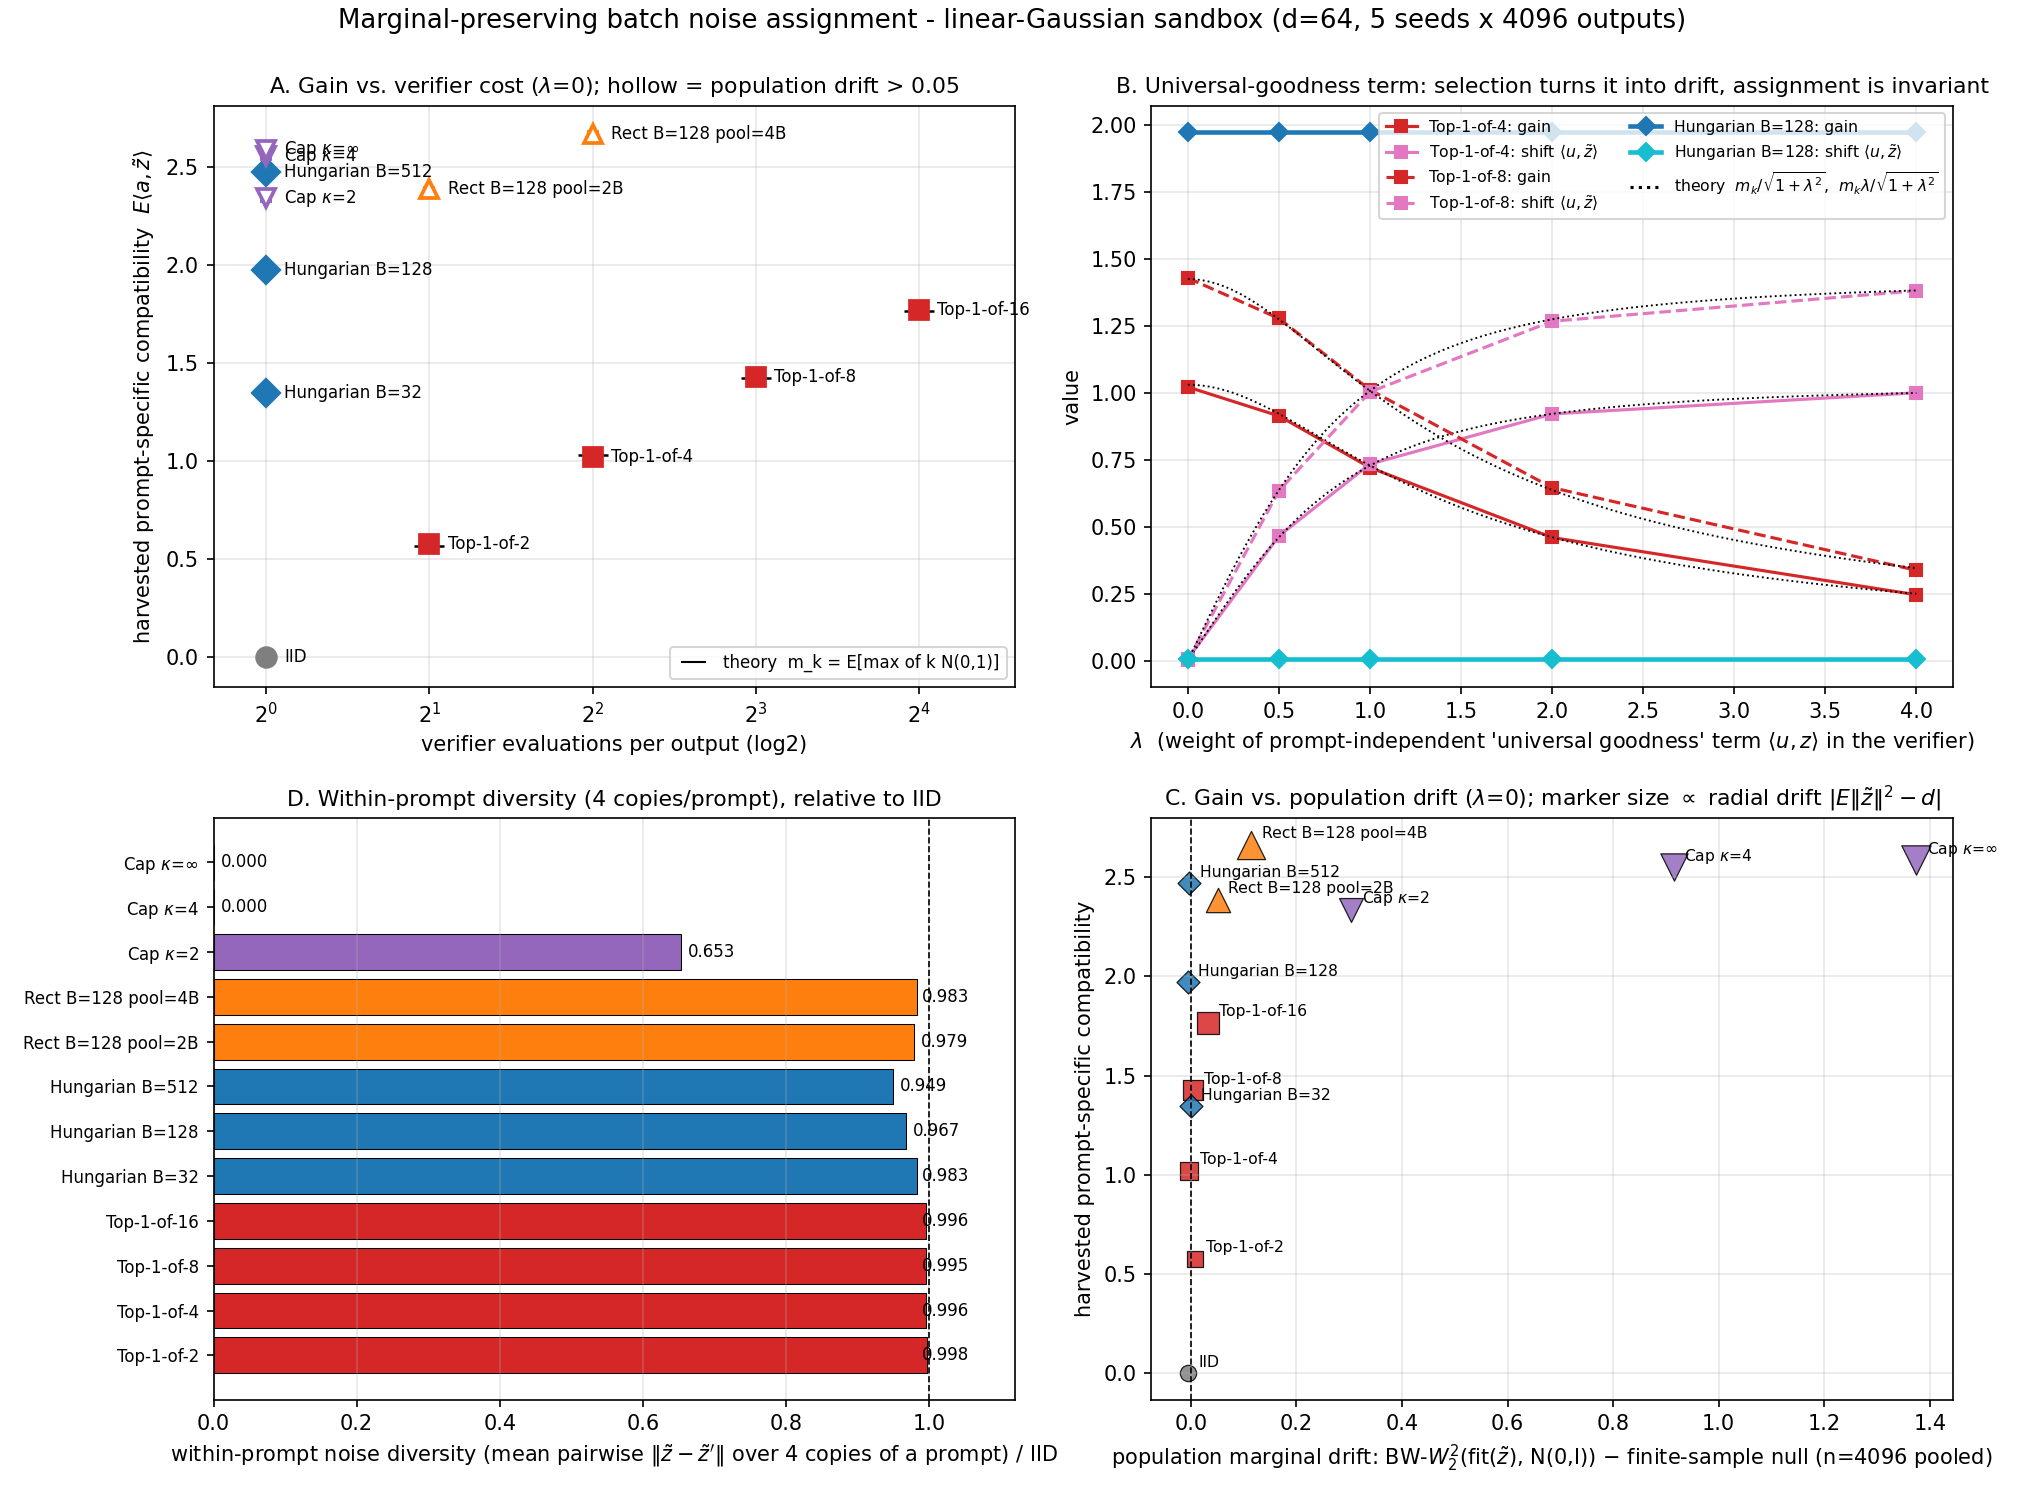
\includegraphics[width=\textwidth]{mpna_sandbox.png}
\end{columns}
\end{frame}

\begin{frame}{MPNA 沙盒：与闭式理论逐点吻合}
\small
\begin{tabular}{lccccc}\toprule
方法（$\lambda{=}0$） & 评分/输出 & 有效增益 & 人口漂移 & 范数漂移 & 同提示多样性 \\ \midrule
IID & 1 & $-0.001$ & 0 & $-0.04$ & 1.000 \\
Top-1-of-4 & 4 & 1.021 & $-0.003$ & $+0.41$ & 0.996 \\
Top-1-of-16 & 16 & 1.768 & $+0.033$ & $+2.42$ & 0.996 \\
\textcolor{ok}{Hungarian $B{=}128$} & \textbf{1} & \textbf{1.972} & \textbf{0（=IID）} & $-0.04$ & 0.967 \\
\textcolor{ok}{Hungarian $B{=}512$} & \textbf{1} & \textbf{2.472} & \textbf{0} & $+0.02$ & 0.949 \\
\textcolor{bad}{共享库检索（$\kappa{=}\infty$）} & 1 & 2.586 & $+1.375$ & $+5.54$ & \textbf{0.000} \\ \bottomrule
\end{tabular}
\vspace{6pt}
\begin{itemize}
\item Top-1-of-4 在 $\lambda=0/0.5/1/2/4$ 的增益 1.021/0.913/0.720/0.459/0.246 vs 理论 $m_4/\sqrt{1+\lambda^2}$ = 1.029/0.921/0.728/0.460/0.250
\item Hungarian $B{=}128$ 以 1 次评分/输出取得等效 top-1-of-25 的增益；5 seeds $\times$ 4096 输出
\end{itemize}
\end{frame}

\begin{frame}{写作红线与下一步}
\begin{columns}
\column{0.5\textwidth}
\textbf{红线}
\begin{itemize}
\item 不说「实现了 OT」，说「以 OT 为目标并度量偏差」
\item 少步比较固定 NFE 口径 + 报告多样性
\item 会议归属官方可核验；预印本一律 [R]
\item 实例级耦合修改必须报告边缘漂移
\end{itemize}
\column{0.5\textwidth}
\textbf{下一步（W3--W4）}
\begin{itemize}
\item MPNA B1 pilot：SDXL-Turbo + GenEval，3 seeds，配漂移套件
\item 复现三件套：Immiscible · OT-CFM · AYS
\item 9/24 NeurIPS 放榜后重跑趋势扫描
\item \#3 漂移度量原型（DDBM / DBIM / CDBM 对照）
\end{itemize}
\end{columns}
\vspace{6pt}
\centering github.com/asimfish/awesome\_diffusion\_OT — README · reports/ · topics/ · papers\_zh/ · report/ · slides/ · trends/
\end{frame}
\end{document}
